\subsection{On the cross-jumped DCB pins}
\label{sec:cross_jumper}
Upon receiving DCB boards, one should notice a pair of (handmade) wire on the
board that cross-jumps the \texttt{J12} configurator pins, as shown in
\autoref{fig:cross_jumper}.

Due to a design oversight, \texttt{SCL} and \texttt{SDA} connections were
flipped, so it has to be cross-jumped.
This will be fixed in final production board.

\begin{figure}[ht]
    \centering
    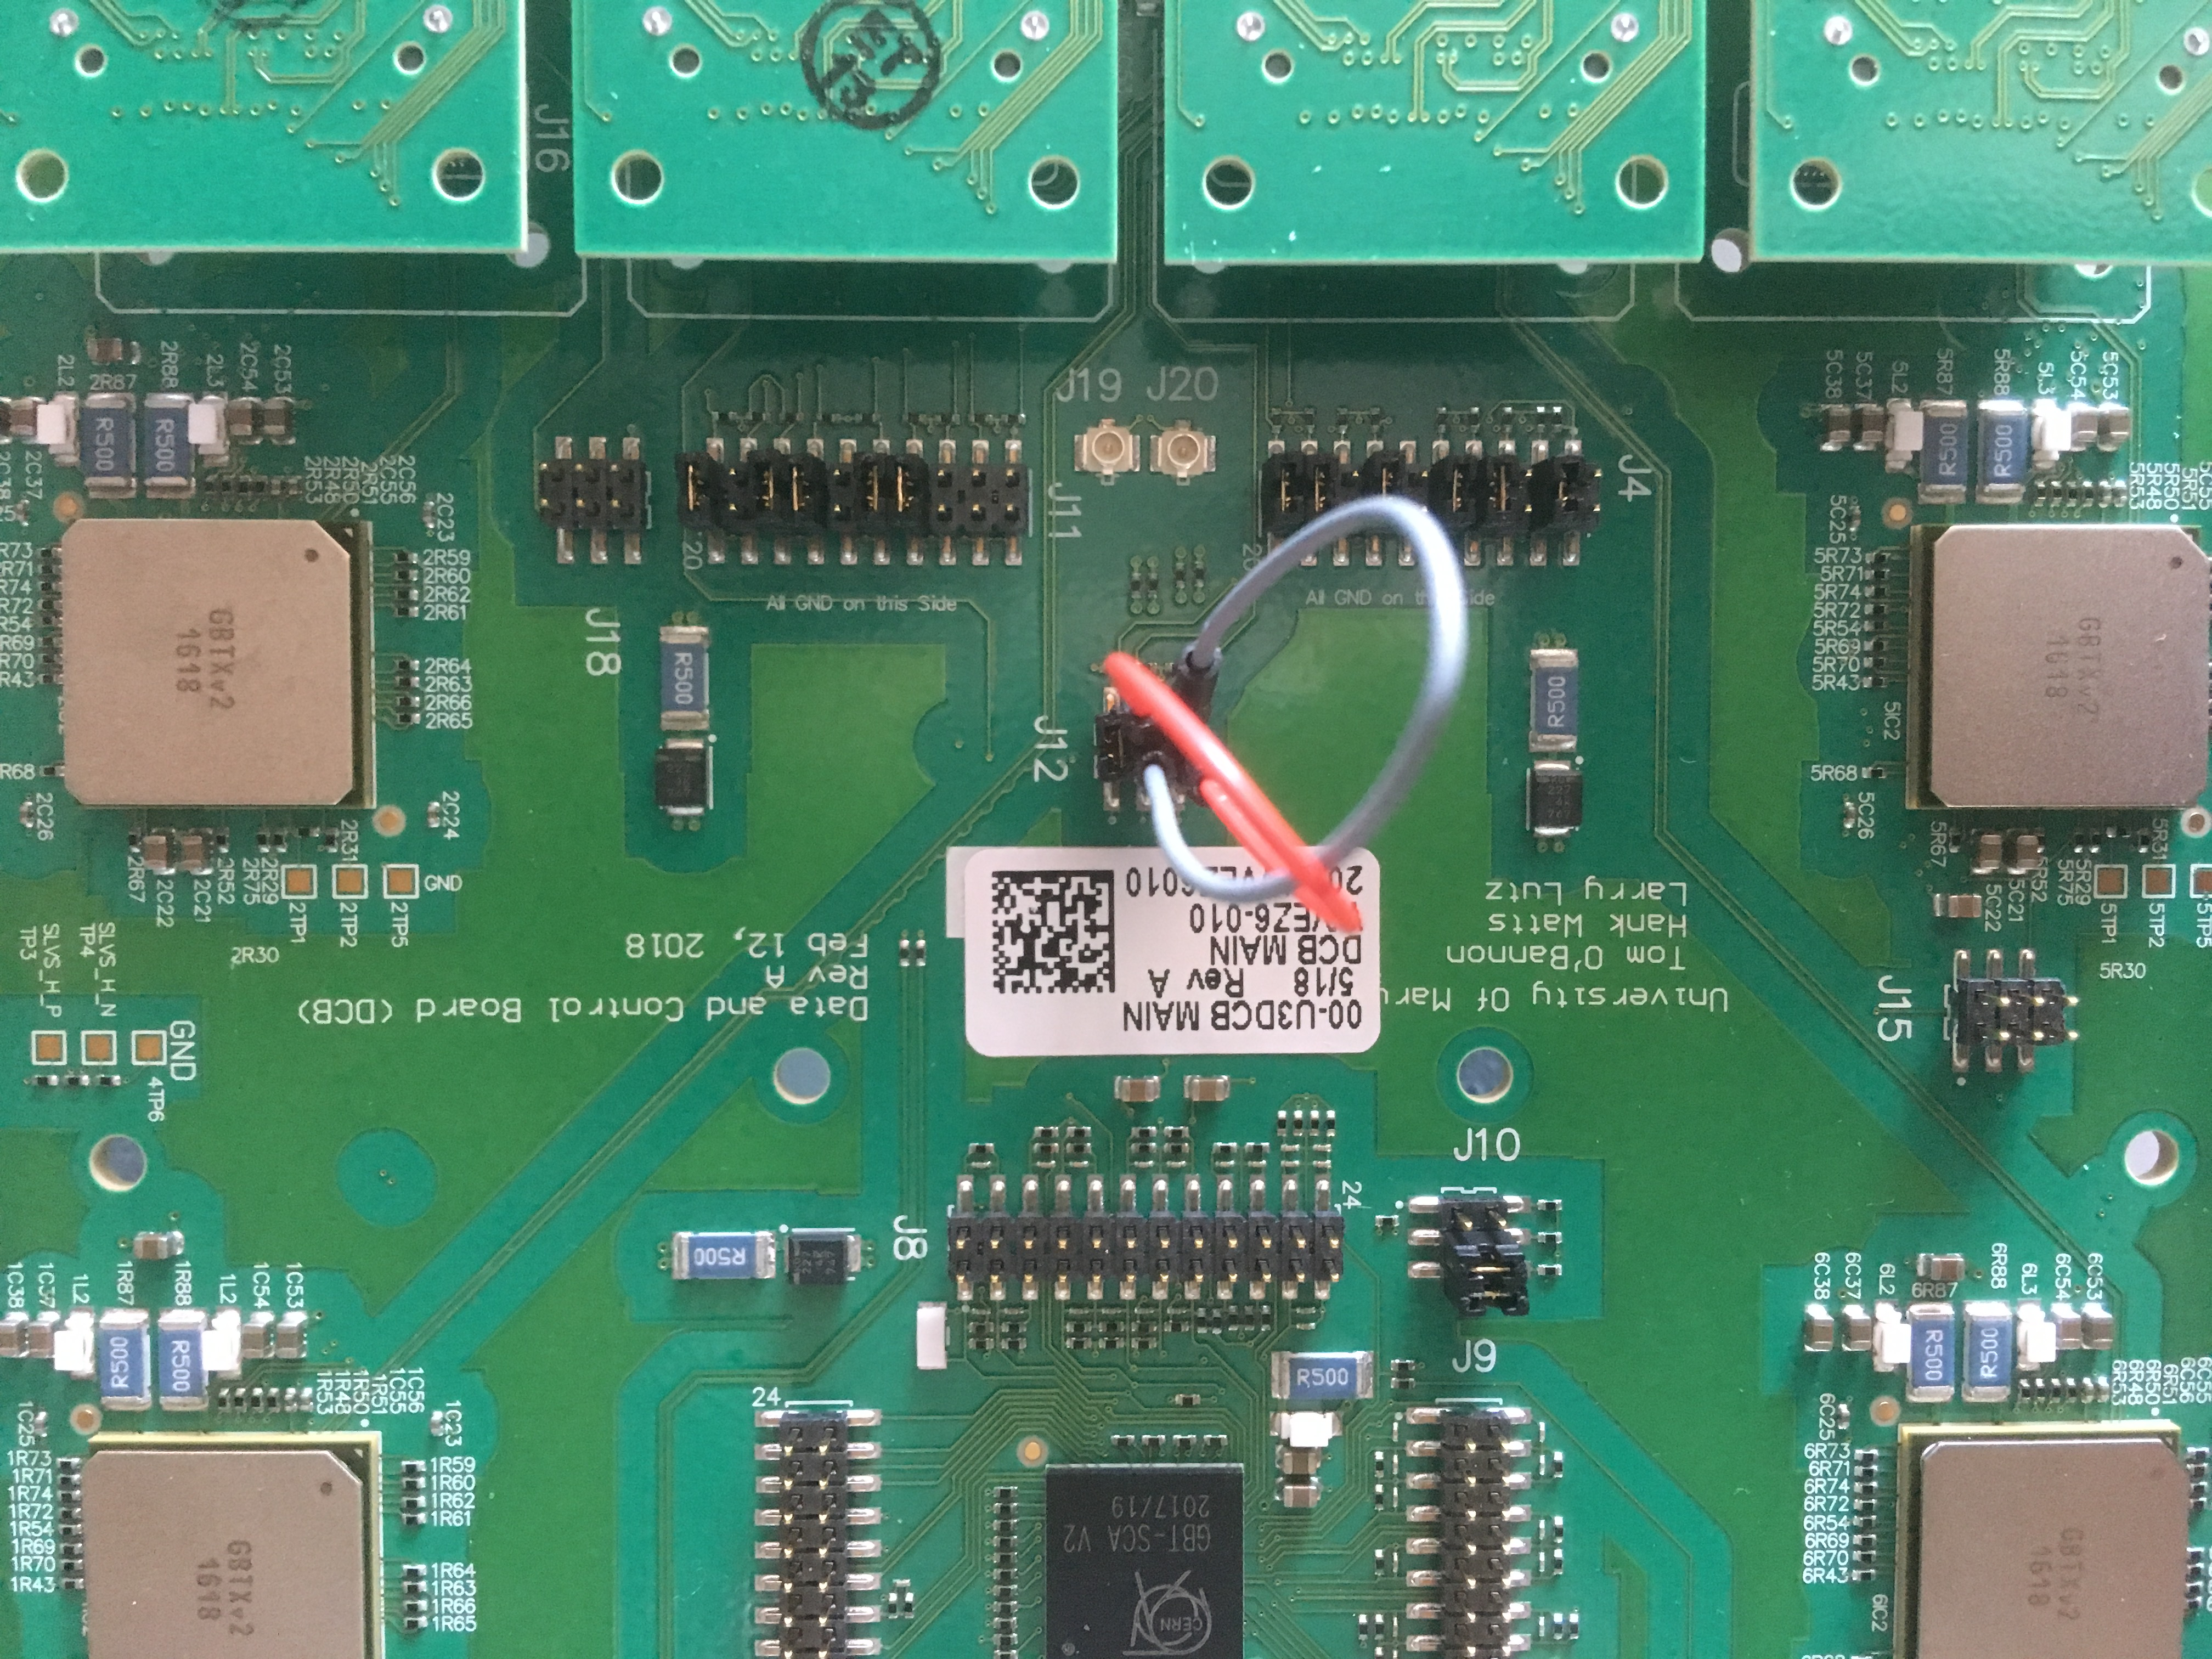
\includegraphics[width=0.9\textwidth]{res/cross_jumper.jpg}
    \caption{Cross-jumped \texttt{J12} pins.}
    \label{fig:cross_jumper}
\end{figure}

\begin{leftbar}
    These cables may fail.
    If one cannot program data GBTxs with GBT client, check the resistance of
    these cables.
\end{leftbar}
